\chapter{Ontology evaluation}
\label{chapter:5_evaluation}

\section{Ontology consistency check}
\label{subsection:5_1_evaluation}
The ontology consistency check consists in running the reasoner in order to check the consistency of declared and inferenced classes and axioms, inferences are made using also SWRL rules described in the encoding section. Running the reasoner ensures also the declaration of disjointness among disjoint classes. I run the HermiT reasoner on both version of the PEO: the version populated manually and the updated version made by GPT-4.\\
On the original version of the PEO, the reasoner does not give any inconsistency and all the axioms are inferred correctly.
\begin{figure}[H]
    \centering
    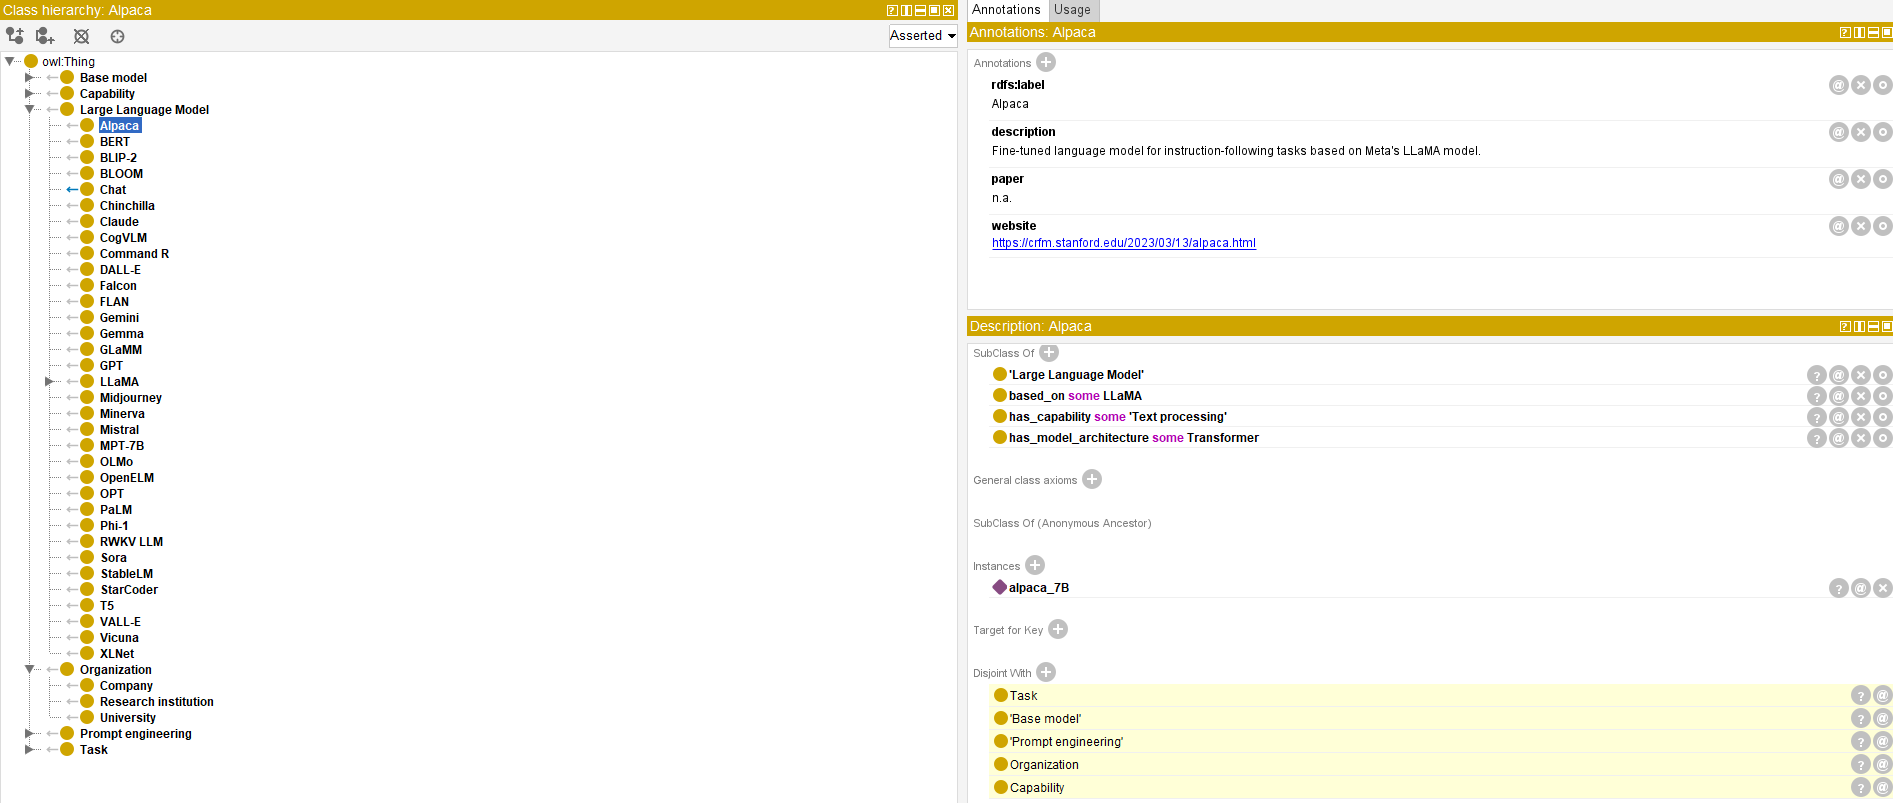
\includegraphics[width=0.9\linewidth]{Figures/fig_39.png}
    \caption{PEO with HermiT reasoner}
    \label{fig:39}
\end{figure}
The Fig. \ref{fig:39} shows the execution of HermiT reasoner on PEO.
The reasoner infers correctly that the class "Alpaca" is disjoint with the classes "Task", "Base model", "Prompt engineering", "Organization" and "Capability" because the superclass "Large language model" is declared disjoint with that list of classes. The ten SWRL rules declared work properly and inference the correct object properties for individuals:
\begin{figure}[H]
    \centering
    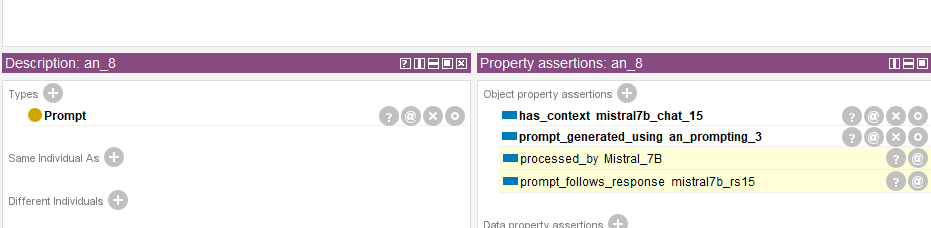
\includegraphics[width=0.9\linewidth]{Figures/fig_40.png}
    \caption{Inference on prompt individual}
    \label{fig:40}
\end{figure}
The consistency check of the other version of the PEO, the one populated using GPT-4 has given the exact results, this because as said in the previous section no additional significant information has been added to the ontology. The inserted classes have no link with other classes so there are no other new inferences.

\subsection{OntoMetrics}
\label{subsection:4_4_2_ontometrics}
The calculation of metrics is done using OntoMetrics: a web-based tool developed by the University of Rostock that validates and provides statistical analyses of ontologies.\cite{lantow2016ontometrics}
Given the ontology in form of RDF file or code, it calculates automatically:
\begin{itemize}
    \item Base metrics: these include simple counts of ontology elements such as classes, axioms, and objects, providing a quantitative overview of the ontology's components.

    \item Schema Metrics: these metrics evaluate the structure of the ontology's schema, considering aspects like attribute richness and inheritance richness.

    \item Knowledge base Metrics: these assess the ontology's knowledge base, focusing on the population of instances within the ontology.

    \item Class Metrics: these metrics analyse individual classes within the ontology, examining factors such as class connectivity and fullness.

    \item Graph Metrics: these evaluate the ontology's taxonomy as a graph, measuring properties like depth and breadth.
\end{itemize}
For PEO, I will calculate base metrics, schema metrics and graph metrics.
\begin{figure}[H]
    \centering
    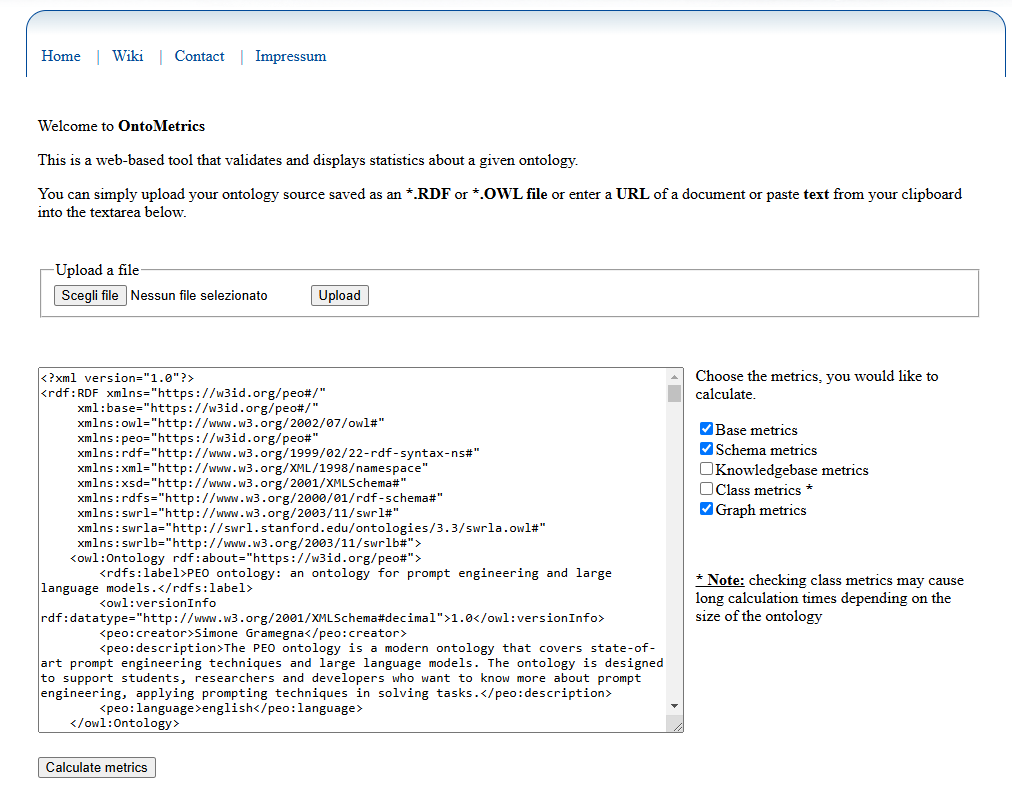
\includegraphics[width=0.9\linewidth]{Figures/fig_41.png}
    \caption{OntoMetrics interface}
    \label{fig:enter-label}
\end{figure}

Values computed for \textbf{base metrics} are:

\begin{table}[H]
    \centering
    \begin{tabular}{|>{\raggedright\arraybackslash}p{8cm}|>{\raggedright\arraybackslash}p{4cm}|}
        \hline
        \textbf{Property} & \textbf{Value} \\ \hline
        Axioms & 2684 \\ \hline
        Logical axioms count & 1695 \\ \hline
        Class count & 126 \\ \hline
        Total classes count & 126 \\ \hline
        Object property count & 34 \\ \hline
        Total object properties count & 34 \\ \hline
        Data property count & 13 \\ \hline
        Total data properties count & 13 \\ \hline
        Properties count & 47 \\ \hline
        Individual count & 352 \\ \hline
        Total individuals count & 352 \\ \hline
        DL expressivity & SRIF(D) \\ \hline
    \end{tabular}
    \caption{PEO base metrics statistics}
    \label{tab:ontology-stats}
\end{table}
This table provides a high-level overview of the ontology’s structure and complexity. With 2684 axioms, the ontology is rich in detail and represents a substantial body of knowledge. Among these, 1695 logical axioms indicate a strong focus on enabling inference and reasoning. The 126 classes show that the ontology has a robust framework for organizing concepts, while 34 object properties and 13 data properties highlight the ontology’s emphasis on relationships over attribute-driven modeling. The inclusion of 352 individuals suggests that the ontology is well-populated, demonstrating practical applicability. The expressivity of SRIF(D) indicates that the ontology supports features like inverse roles and data ranges, balancing computational efficiency with expressive capability. This ontology is comprehensive but may require optimization to handle its inherent complexity effectively.

\begin{table}[H]
    \centering
    \begin{tabular}{|>{\raggedright\arraybackslash}p{8cm}|>{\raggedright\arraybackslash}p{4cm}|}
        \hline
        \textbf{Class Axiom Type} & \textbf{Count} \\ \hline
        SubClassOf axioms count & 199 \\ \hline
        Equivalent classes axioms count & 1 \\ \hline
        Disjoint classes axioms count & 3 \\ \hline
        GCICount & 0 \\ \hline
        HiddenGCICount & 0 \\ \hline
    \end{tabular}
    \caption{PEO Class Axioms statistics}
    \label{tab:class-axioms}
\end{table}

This table details how classes are defined and interrelated within the ontology. The 199 SubClassOf axioms form a strong hierarchical backbone, enabling inheritance of properties and constraints. However, the limited use of equivalent classes (1) and disjoint classes (3) suggests that the ontology may not fully capture nuanced relationships or enforce strict separations between certain concepts. The absence of GCIs (Global Cardinality Restrictions) and Hidden GCIs could indicate missed opportunities to model constraints and relationships that extend across the ontology as a whole. While the current setup simplifies reasoning, incorporating more advanced axioms could enhance the ontology's semantic richness and utility.


\begin{table}[H]
    \centering
    \begin{tabular}{|>{\raggedright\arraybackslash}p{8cm}|>{\raggedright\arraybackslash}p{4cm}|}
        \hline
        \textbf{Object Property Axiom Type} & \textbf{Count} \\ \hline
        SubObjectPropertyOf axioms count & 33 \\ \hline
        Equivalent object properties axioms count & 0 \\ \hline
        Inverse object properties axioms count & 16 \\ \hline
        Disjoint object properties axioms count & 0 \\ \hline
        Functional object properties axioms count & 0 \\ \hline
        Inverse functional object properties axioms count & 0 \\ \hline
        Transitive object property axioms count & 2 \\ \hline
        Symmetric object property axioms count & 0 \\ \hline
        Asymmetric object property axioms count & 0 \\ \hline
        Reflexive object property axioms count & 0 \\ \hline
        Irreflexive object property axioms count & 1 \\ \hline
        Object property domain axioms count & 33 \\ \hline
        Object property range axioms count & 33 \\ \hline
        SubPropertyChainOf axioms count & 0 \\ \hline
    \end{tabular}
    \caption{PEO Object Property Axioms Statistics}
    \label{tab:object-property-axioms}
\end{table}
Object properties are the backbone of the ontology's relational structure. With 33 SubObjectPropertyOf axioms, the ontology defines a clear hierarchy of relationships, which helps maintain organization and reasoning efficiency. The 16 inverse object properties highlight a good use of bidirectional relationships, enhancing navigability within the graph. However, the lack of functional, inverse functional, symmetric, or asymmetric properties may limit the ontology’s ability to capture specific constraints, such as unique or one-to-one relationships. The two transitive properties and one irreflexive property add some complexity but are underused. Domains and ranges are well-defined for all object properties, which is a strong point, as it ensures consistency and logical soundness in property usage.

\begin{table}[H]
    \centering
    \begin{tabular}{|>{\raggedright\arraybackslash}p{8cm}|>{\raggedright\arraybackslash}p{4cm}|}
        \hline
        \textbf{Data Property Axiom Type} & \textbf{Count} \\ \hline
        SubDataPropertyOf axioms count & 12 \\ \hline
        Equivalent data properties axioms count & 0 \\ \hline
        Disjoint data properties axioms count & 0 \\ \hline
        Functional data property axioms count & 7 \\ \hline
        Data property domain axioms count & 11 \\ \hline
        Data property range axioms count & 12 \\ \hline
    \end{tabular}
    \caption{PEO Data Property Axioms Statistics}
    \label{tab:data-property-axioms}
\end{table}

Data properties focus on attributes of individuals. The 12 SubDataPropertyOf axioms indicate some level of organization, but the absence of equivalent or disjoint data properties suggests limited semantic relationships among these properties. Seven functional data properties point to a partial emphasis on ensuring that certain attributes have unique values (e.g., “hasID”), but this aspect could be expanded. Domains and ranges are defined for most properties, which improves clarity and reasoning, but the relatively low overall count of data property axioms might limit the ontology's ability to model detailed attributes of classes or individuals.

\begin{table}[H]
    \centering
    \begin{tabular}{|>{\raggedright\arraybackslash}p{8cm}|>{\raggedright\arraybackslash}p{4cm}|}
        \hline
        \textbf{Individual Axiom Type} & \textbf{Count} \\ \hline
        Class assertion axioms count & 352 \\ \hline
        Object property assertion axioms count & 390 \\ \hline
        Data property assertion axioms count & 580 \\ \hline
        Negative object property assertion axioms count & 0 \\ \hline
        Negative data property assertion axioms count & 0 \\ \hline
        Same individuals axioms count & 0 \\ \hline
        Different individuals axioms count & 0 \\ \hline
    \end{tabular}
    \caption{PEO Individual Axioms Statistics}
    \label{tab:individual-axioms}
\end{table}

This table reflects how individuals are represented and connected within the ontology. The 352 class assertions and 390 object property assertions indicate that the ontology’s individuals are well-categorized and interlinked. The 580 data property assertions further show that these individuals have descriptive attributes. However, the absence of negative assertions (both object and data properties) and no axioms for declaring individuals as equivalent or distinct may limit the ontology's ability to handle complex scenarios, such as resolving conflicts or managing redundancy.

\begin{table}[H]
    \centering
    \begin{tabular}{|>{\raggedright\arraybackslash}p{8cm}|>{\raggedright\arraybackslash}p{4cm}|}
        \hline
        \textbf{Annotation Axiom Type} & \textbf{Count} \\ \hline
        Annotation axioms count & 5 \\ \hline
        Annotation assertion axioms count & 459 \\ \hline
        Annotation property domain axioms count & 0 \\ \hline
        Annotation property range axioms count & 0 \\ \hline
    \end{tabular}
    \caption{PEO Annotation Axioms Statistics}
    \label{tab:annotation-axioms}
\end{table}
Annotations are crucial for documentation and understanding. With 459 annotation assertions, the ontology appears well-documented, providing metadata that can improve usability and comprehension. However, the absence of domain and range axioms for annotation properties suggests that these annotations are not constrained formally, which could lead to inconsistencies or reduced clarity in large-scale applications. Better structuring of annotation properties could enhance the ontology’s maintainability.\\
The \textbf{Schema metrics} computed for PEO are: 

\begin{table}[H]
    \centering
    \begin{tabular}{|>{\raggedright\arraybackslash}p{8cm}|>{\raggedright\arraybackslash}p{4cm}|}
        \hline
        \textbf{Metric} & \textbf{Value} \\ \hline
        Attribute richness & 0.103175 \\ \hline
        Inheritance richness & 1.579365 \\ \hline
        Relationship richness & 0.160338 \\ \hline
        Attribute class ratio & 0.0 \\ \hline
        Equivalence ratio & 0.007937 \\ \hline
        Axiom/class ratio & 21.301587 \\ \hline
        Inverse relations ratio & 0.390244 \\ \hline
        Class/relation ratio & 0.531646 \\ \hline
    \end{tabular}
    \caption{PEO Schema Metrics}
    \label{tab:ontology-metrics}
\end{table}
This table evaluates the structural aspects of the ontology. The attribute richness (0.103175) indicates that relatively few classes have associated attributes, which could limit the detail available for each class. The inheritance richness (1.579365) shows that most classes are part of meaningful hierarchies, a positive sign of structure. However, the relationship richness (0.160338) is relatively low, suggesting that the ontology focuses more on defining concepts than on interconnecting them. The axiom-to-class ratio (21.301587) highlights a dense ontology, meaning each class has substantial associated information, which can be both a strength and a source of complexity. Finally, the inverse relations ratio (0.390244) indicates a good but incomplete use of inverse properties to enhance navigability.\\
The \textbf{Graph metrics} for PEO are:
\begin{table}[H]
    \centering
    \begin{tabular}{|>{\raggedright\arraybackslash}p{8cm}|>{\raggedright\arraybackslash}p{4cm}|}
        \hline
        \textbf{Metric} & \textbf{Value} \\ \hline
        Absolute root cardinality & 7 \\ \hline
        Absolute leaf cardinality & 109 \\ \hline
        Absolute sibling cardinality & 126 \\ \hline
        Absolute depth & 318 \\ \hline
        Average depth & 2.52381 \\ \hline
        Maximal depth & 4 \\ \hline
        Absolute breadth & 126 \\ \hline
        Average breadth & 7.0 \\ \hline
        Maximal breadth & 33 \\ \hline
        Ratio of leaf fan-outness & 0.865079 \\ \hline
        Ratio of sibling fan-outness & 1.0 \\ \hline
        Tangledness & 0.269841 \\ \hline
        Total number of paths & 126 \\ \hline
        Average number of paths & 31.5 \\ \hline
    \end{tabular}
    \caption{PEO Graph Metrics}
    \label{tab:cardinality-depth-metrics}
\end{table}
Graph metrics provide insights into the topology of the ontology. The absolute root cardinality (7) and absolute leaf cardinality (109) indicate a moderately deep hierarchy with good granularity at the leaf level. The maximal depth (4) and average depth (2.52381) suggest a shallow graph, which can make the ontology easier to understand but may oversimplify complex domains. The tangledness (0.269841) is moderate, indicating a graph structure that is connected but not overly complex. The high sibling fan-out ratio (1.0) shows that sibling classes are evenly distributed, while the ratio of leaf fan-outness (0.865079) implies a balanced spread of subclasses from intermediate nodes.\\
Despite there being no significant differences between the original version of the PEO and the version populated using GPT-4, I proceed to calculate metrics.\\
Values computed for base metrics are:
\begin{table}[H]
    \centering
    \begin{tabular}{|>{\raggedright\arraybackslash}p{8cm}|>{\raggedright\arraybackslash}p{4cm}|}
        \hline
        \textbf{Property} & \textbf{Value} \\ \hline
        Axioms & 2705 \\ \hline
        Logical axioms count & 1710 \\ \hline
        Class count & 128 \\ \hline
        Total classes count & 128 \\ \hline
        Object property count & 34 \\ \hline
        Total object properties count & 34 \\ \hline
        Data property count & 13 \\ \hline
        Total data properties count & 13 \\ \hline
        Properties count & 47 \\ \hline
        Individual count & 359 \\ \hline
        Total individuals count & 359 \\ \hline
        DL expressivity & SRIF(D) \\ \hline
    \end{tabular}
    \caption{PEO updated base metrics statistics}
    \label{tab:ontology-stats-updated}
\end{table}

\begin{table}[H]
    \centering
    \begin{tabular}{|>{\raggedright\arraybackslash}p{8cm}|>{\raggedright\arraybackslash}p{4cm}|}
        \hline
        \textbf{Class Axiom Type} & \textbf{Count} \\ \hline
        SubClassOf axioms count & 197 \\ \hline
        Equivalent classes axioms count & 1 \\ \hline
        Disjoint classes axioms count & 3 \\ \hline
        GCICount & 0 \\ \hline
        HiddenGCICount & 0 \\ \hline
    \end{tabular}
    \caption{PEO updated Class Axioms Statistics}
    \label{tab:class-axioms-updated}
\end{table}

\begin{table}[H]
    \centering
    \begin{tabular}{|>{\raggedright\arraybackslash}p{8cm}|>{\raggedright\arraybackslash}p{4cm}|}
        \hline
        \textbf{Object Property Axiom Type} & \textbf{Count} \\ \hline
        SubObjectPropertyOf axioms count & 33 \\ \hline
        Equivalent object properties axioms count & 0 \\ \hline
        Inverse object properties axioms count & 16 \\ \hline
        Disjoint object properties axioms count & 0 \\ \hline
        Functional object properties axioms count & 0 \\ \hline
        Inverse functional object properties axioms count & 0 \\ \hline
        Transitive object property axioms count & 8 \\ \hline
        Symmetric object property axioms count & 1 \\ \hline
        Asymmetric object property axioms count & 0 \\ \hline
        Reflexive object property axioms count & 0 \\ \hline
        Irreflexive object property axioms count & 1 \\ \hline
        Object property domain axioms count & 33 \\ \hline
        Object property range axioms count & 33 \\ \hline
        SubPropertyChainOf axioms count & 0 \\ \hline
    \end{tabular}
    \caption{PEO updated Object Property Axioms Statistics}
    \label{tab:object-property-axioms-updated}
\end{table}

\begin{table}[H]
    \centering
    \begin{tabular}{|>{\raggedright\arraybackslash}p{8cm}|>{\raggedright\arraybackslash}p{4cm}|}
        \hline
        \textbf{Data Property Axiom Type} & \textbf{Count} \\ \hline
        SubDataPropertyOf axioms count & 12 \\ \hline
        Equivalent data properties axioms count & 0 \\ \hline
        Disjoint data properties axioms count & 0 \\ \hline
        Functional data property axioms count & 7 \\ \hline
        Data property domain axioms count & 12 \\ \hline
        Data property range axioms count & 12 \\ \hline
    \end{tabular}
    \caption{PEO updated Data Property Axioms Statistics}
    \label{tab:data-property-axioms-updated}
\end{table}

\begin{table}[H]
    \centering
    \begin{tabular}{|>{\raggedright\arraybackslash}p{8cm}|>{\raggedright\arraybackslash}p{4cm}|}
        \hline
        \textbf{Individual Axiom Type} & \textbf{Count} \\ \hline
        Class assertion axioms count & 358 \\ \hline
        Object property assertion axioms count & 393 \\ \hline
        Data property assertion axioms count & 580 \\ \hline
        Negative object property assertion axioms count & 0 \\ \hline
        Negative data property assertion axioms count & 0 \\ \hline
        Same individuals axioms count & 0 \\ \hline
        Different individuals axioms count & 0 \\ \hline
    \end{tabular}
    \caption{PEO updated Individual Axioms Statistics}
    \label{tab:individual-axioms-updated}
\end{table}

\begin{table}[H]
    \centering
    \begin{tabular}{|>{\raggedright\arraybackslash}p{8cm}|>{\raggedright\arraybackslash}p{4cm}|}
        \hline
        \textbf{Annotation Axiom Type} & \textbf{Count} \\ \hline
        Annotation axioms count & 5 \\ \hline
        Annotation assertion axioms count & 456 \\ \hline
        Annotation property domain axioms count & 0 \\ \hline
        Annotation property range axioms count & 0 \\ \hline
    \end{tabular}
    \caption{PEO updated Annotation Axioms Statistics}
    \label{tab:annotation-axioms-updated}
\end{table}

The schema metrics for the update version of PEO are:
\begin{table}[H]
    \centering
    \begin{tabular}{|>{\raggedright\arraybackslash}p{8cm}|>{\raggedright\arraybackslash}p{4cm}|}
        \hline
        \textbf{Metric} & \textbf{Value} \\ \hline
        Attribute richness & 0.101563 \\ \hline
        Inheritance richness & 1.539063 \\ \hline
        Relationship richness & 0.161702 \\ \hline
        Attribute class ratio & 0.0 \\ \hline
        Equivalence ratio & 0.007813 \\ \hline
        Axiom/class ratio & 21.132813 \\ \hline
        Inverse relations ratio & 0.390244 \\ \hline
        Class/relation ratio & 0.544681 \\ \hline
    \end{tabular}
    \caption{PEO Schema Metrics}
    \label{tab:ontology-metrics-updated}
\end{table}

The graph metrics for updated version of PEO are:

\begin{table}[H]
    \centering
    \begin{tabular}{|>{\raggedright\arraybackslash}p{8cm}|>{\raggedright\arraybackslash}p{4cm}|}
        \hline
        \textbf{Metric} & \textbf{Value} \\ \hline
        Absolute root cardinality & 11 \\ \hline
        Absolute leaf cardinality & 111 \\ \hline
        Absolute sibling cardinality & 128 \\ \hline
        Absolute depth & 316 \\ \hline
        Average depth & 2.46875 \\ \hline
        Maximal depth & 4 \\ \hline
        Absolute breadth & 128 \\ \hline
        Average breadth & 7.111111 \\ \hline
        Maximal breadth & 33 \\ \hline
        Ratio of leaf fan-outness & 0.867188 \\ \hline
        Ratio of sibling fan-outness & 1.0 \\ \hline
        Tangledness & 0.265625 \\ \hline
        Total number of paths & 128 \\ \hline
        Average number of paths & 32.0 \\ \hline
    \end{tabular}
    \caption{PEO updated Graph Metrics}
    \label{tab:cardinality-depth-metrics-updated}
\end{table}
The new values calculated by OntoMetrics on the updated version of the ontology do not differ significantly from the previously calculated values, as the large language model GPT-4 has only added four new classes and three new instances. All results for PEO and its second version are on \href{https://github.com/simonegramegna/peo/tree/main/evaluation}{Github}.

\newpage
\subsection{OOPS! validation}
\label{subsection:4_4_3_oops}
The methods discussed so far are widely used in ontology evaluation; however, they are not capable of capturing modelling errors in greater detail. These errors can compromise not only the quality and usability of the ontology but also lead to potential inconsistencies. Therefore, it is necessary to adopt a different approach from those previously examined, OntoMetrics and the HermiT reasoner because they have the following issues:
\begin{itemize}
    \item OntoMetrics: it provides a quantitative measure of ontology's structural characteristics without analysing qualitative aspects, so it is not able to detect semantic and usability issues in the ontology.

    \item HermiT reasoner (reasoners in general): reasoners are designed to check the logical consistency of an ontology and perform inferencing identifying inconsistencies in axioms. But reasoners are not able to detect errors outside logical inconsistencies, such as missing domain or range definitions and they cannot check best-practice violation and usability issues.
\end{itemize}
These limitations highlight the need for a tool that can go beyond structural and logical evaluation, addressing both semantic and usability dimensions of ontology quality. \textbf{OOPS!} (Ontology Pitfall Scanner) is an online tool for ontology evaluation \cite{poveda2014oops} that automates the evaluation process without requiring any effort by the developer. 
\begin{figure}[H]
    \centering
    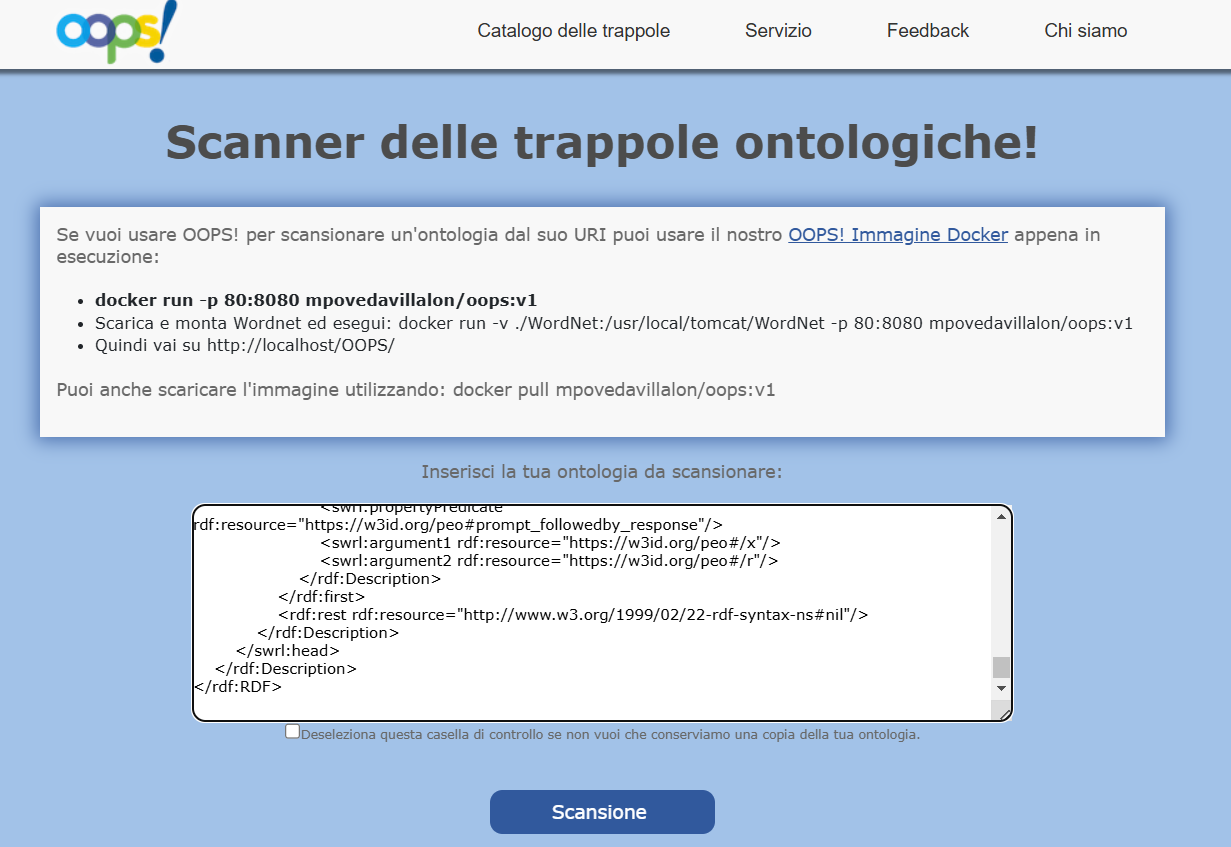
\includegraphics[width=0.9\linewidth]{Figures/fig_42.png}
    \caption{OOPS! web interface}
    \label{fig:enter-label}
\end{figure}
Given the input ontology, OOPS is able to detect 40 different pitfall that are classified into three categories: critical, important and minor by parsing the RDF code and generating a complete response using the OOPS! scanner. Pitfalls in the scanner include:
\begin{itemize}
    \item Structural pitfalls: these involve issues related to the ontology's formal structure and syntax like cycles in hierarchy and unconnected ontology elements.

    \item Functional pitfalls: these involve issues to the intended use and functionality of the ontology like missing domain or incorrectly defined inverse relationships.

    \item Usability and Profiling Pitfalls: these involve issues  affecting the ontology's clarity, maintainability, and human-readability like missing annotations, inconsistent naming and ambiguous terms.
\end{itemize}
I will use OOPS! scanner on both versions of the PEO detecting and explaining found pitfalls. 
For the first version of PEO there are just three pitfalls:
\begin{figure}[H]
    \centering
    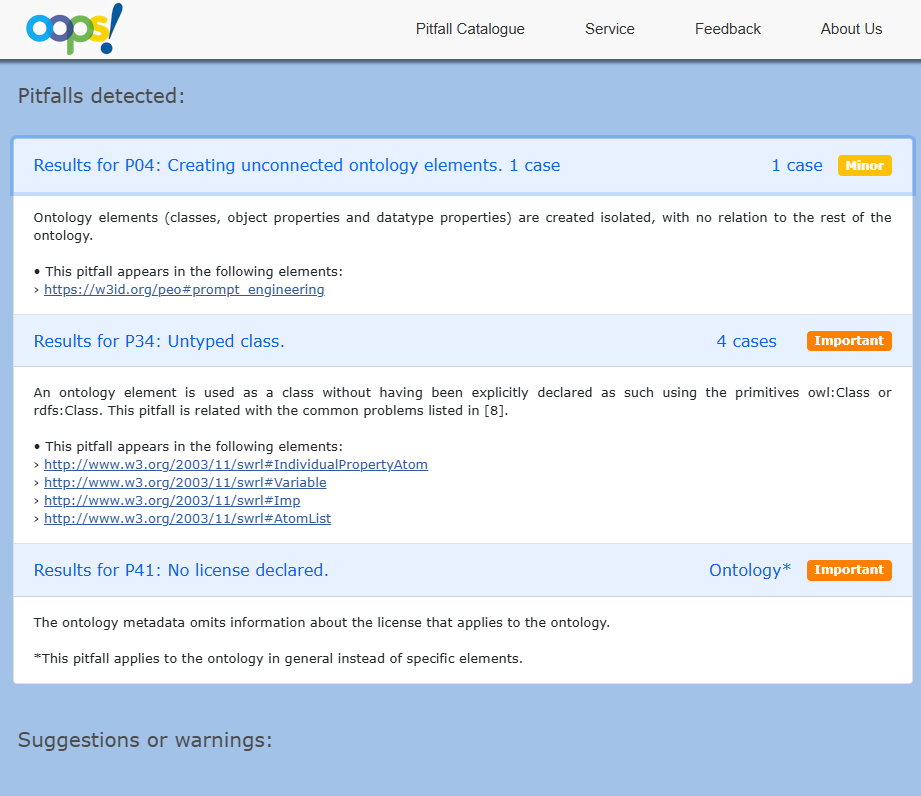
\includegraphics[width=0.9\linewidth]{Figures/fig_43.png}
    \caption{Detected pitfalls PEO}
    \label{fig:enter-label}
\end{figure}
The explanation of detected pitfall is:
\begin{itemize}
    \item \textbf{P04 (Creating unconnected ontology elements):} this pitfall involves ontology elements (classes, object properties and datatype properties) are created isolated, with no relation to the rest of the ontology. 

    \item \textbf{P34 (Untyped class):} this pitfalls involves all ontology elements that are used as a class without having explicitly declared. This pitfall involves four elements in PEO: \\ \textit{http://www.w3.org/2003/11/swrl\#IndividualPropertyAtom},\\ \textit{http://www.w3.org/2003/11/swrl\#Variable},\\ \textit{http://www.w3.org/2003/11/swrl\#Imp} and \\\textit{http://www.w3.org/2003/11/swrl\#AtomList}.

    \item \textbf{P41 (No license declared):} there is no license in the ontology metadata.    
\end{itemize}
Overall, the report is satisfactory, as no critical pitfalls have been identified, nor any issues found in the main classes or object properties of the ontology and I will discuss in more detail in Results discussion section. The complete report is available \href{https://github.com/simonegramegna/peo/blob/main/evaluation/oops_report_peo.xml}{here}. After detecting pitfalls in the original version of the PEO, I also examined the populated version generated using GPT-4 nonetheless, no significant differences were observed between the two versions. Compared to the three pitfalls identified in the previous version, OOPS detects five pitfalls:
\begin{figure}[H]
    \centering
    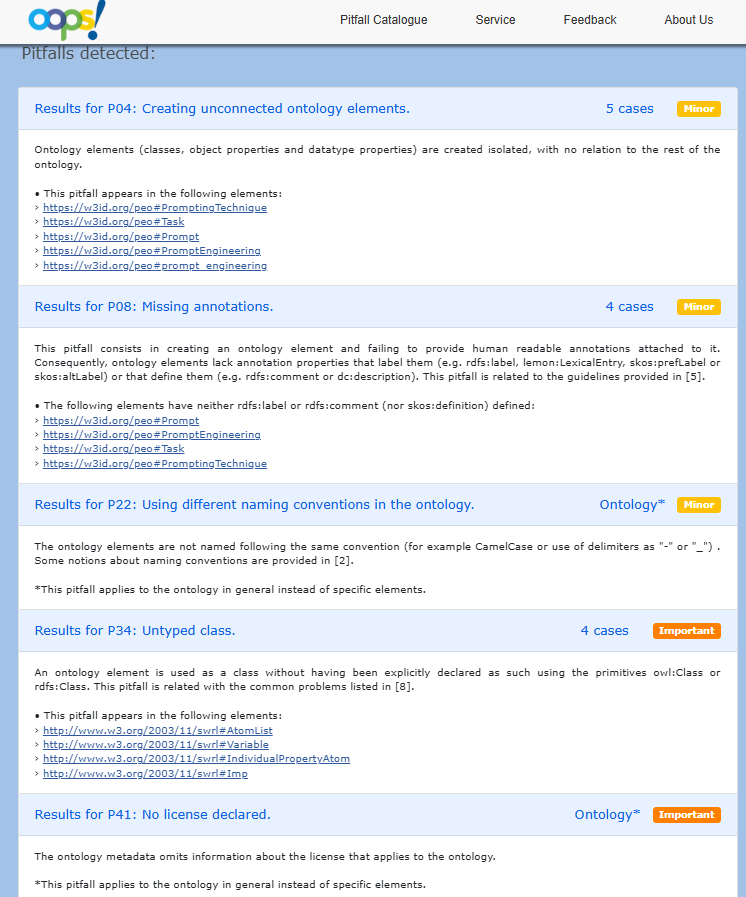
\includegraphics[width=0.75\linewidth]{Figures/fig_44.png}
    \caption{Detected pitfalls second version PEO}
    \label{fig:enter-label}
\end{figure}


\begin{itemize}
    \item \textbf{P04 (Creating unconnected ontology elements):} this pitfall, as said before, involves unconnected ontology elements. This time the pitfall involves not only the \textit{prompt\_engineering} class but also the new classes created by GPT-4: \textit{Task}, \textit{PromptingTechnique}, \textit{Prompt} and \textit{PromptEngineering}. Those classes have no relations with other classes.

    \item \textbf{P08 (Missing annotations):} this pitfall involves elements that lack annotation properties that label them ( \textit{rdfs:label}) or that define them\\ (\textit{rdfs:comment}). This pitall involves the four classes created by GPT-4 with no comment provided: \textit{Task}, \textit{PromptingTechnique}, \textit{Prompt} and \textit{PromptEngineering}.  

    \item \textbf{P22 (Using different naming conventions in the ontology):} this pitfall involves ontology elements are not named following the same convention (for example CamelCase or use of delimiters as "-" or "\_"). This pitfall is given by the new classes created by GPT-4 that do not follow the naming convention used in the ontology (with the "\_" separator) by creating classes declared in camel case.

    \item \textbf{P34 (Untyped class):} this is the same pitfall detected before.

    \item \textbf{P41 (No license declared):} this is the same pitfall detected before.
\end{itemize}
In general, the detected pitfalls are caused by GPT-4's lack of understanding of the ontology's structure and I will discuss in more detail in the Results discussion section. The oops report is available \href{https://github.com/simonegramegna/peo/blob/main/evaluation/oops_report_peo_gpt4.xml}{here}.


\subsection{SPARQL queries}
\label{subsection:4_4_4_sparql}
The final step of ontology evaluation is converting competency questions (CQ) defined in the \textit{Ontology requirements specification} section into SPARQL queries in order to compare the expected result to the actual result of each competency question. SPARQL queries are generated manually and ran using Jupyter notebook \cite{jupyter}: an enviroment for running python code and the rdflib python library \cite{rdflib}: a library to access rdf files and run SPARQL queries inside python. The code is available on the \href{https://github.com/simonegramegna/peo/tree/main/evaluation}{Github repository} and the evaluation is mode for both versions of the ontology.\\
First I open the ontology using rdflib:
\begin{figure}[H]
    \centering
    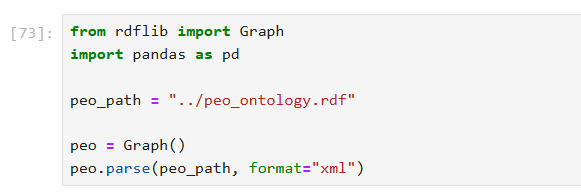
\includegraphics[width=0.9\linewidth]{Figures/fig_45.png}
    \caption{Jupyter notebook SPARQL}
    \label{fig:enter-label}
\end{figure}
The pandas library is used to display query results in data-frames, for query and display I created three support functions: 
\begin{itemize}
    \item \textit{execute\_query:} it takes as input the SPARQL query string and returns a list of results.

    \item \textit{results\_to\_df:} it takes as input as input the list of results ad creates and returns a dataframe with results inside which columns' names are the label names.

    \item \textit{print\_results:} it iterates on the list of results and prints each element.
\end{itemize}
We can see the implementation below:
\begin{figure}[H]
    \centering
    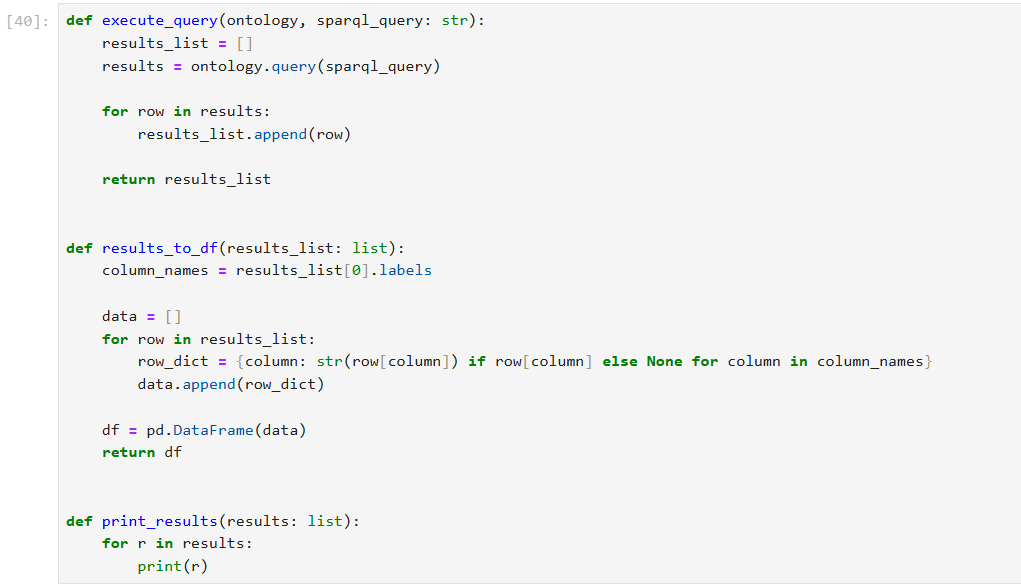
\includegraphics[width=0.9\linewidth]{Figures/fig_46.png}
    \caption{Support python functions}
    \label{fig:enter-label}
\end{figure}

Once this is done, I can translate each of the sixteen competency questions into SPARQL queries to be executed on PEO.\\
The first competency question \textbf{CQ1: What is prompt engineering?} is translated into:
\begin{lstlisting}
    SELECT DISTINCT ?property ?value
    WHERE {
        <https://w3id.org/peo#prompt_engineering> ?property ?value .
    }
\end{lstlisting}
Getting the following result:
\begin{figure}[H]
    \centering
    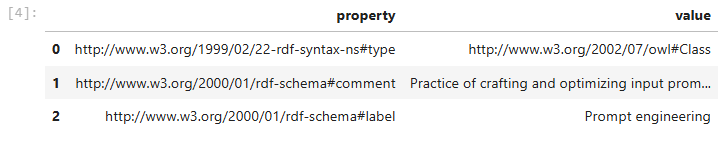
\includegraphics[width=0.9\linewidth]{Figures/fig_47.png}
    \caption{CQ1 SPARQL query results}
    \label{fig:enter-label}
\end{figure}
The output from the query matches the expected result, which is the definition of prompt engineering.\\

The second competency question \textbf{CQ2: What is a prompt?} is translated into:
\begin{lstlisting}
SELECT DISTINCT ?property ?value
WHERE {
    <https://w3id.org/peo#prompt> ?property ?value .
}
\end{lstlisting}
Getting the following results:
\begin{figure}[H]
    \centering
    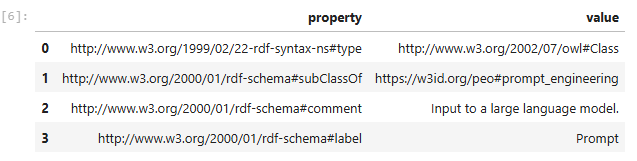
\includegraphics[width=0.9\linewidth]{Figures/fig_48.png}
    \caption{CQ2 SPARQL query results}
    \label{fig:enter-label}
\end{figure}

The output also in this case matches the expected result, which is the definition of prompt.\\

The third competency question \textbf{CQ3: What are prompting techniques?} is translated into:
\begin{lstlisting}
SELECT DISTINCT ?subclass ?label
WHERE {
    ?subclass rdfs:subClassOf <https://w3id.org/peo#prompting_technique> .
    OPTIONAL { ?subclass rdfs:label ?label . }
}
\end{lstlisting}
Getting the following results:
\begin{figure}[H]
    \centering
    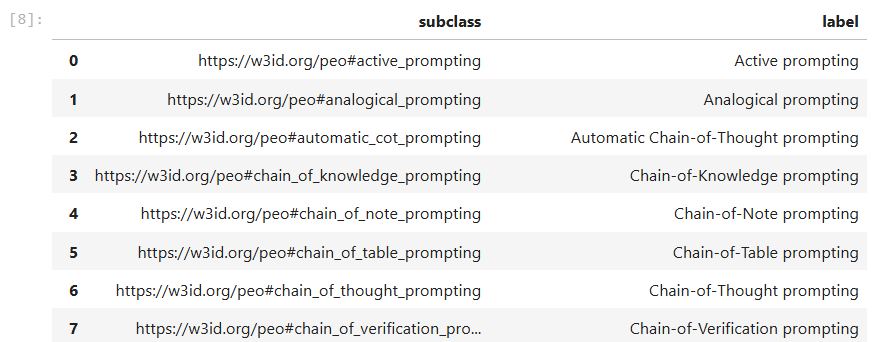
\includegraphics[width=0.9\linewidth]{Figures/fig_49.png}
    \caption{CQ3 SPARQL query results}
    \label{fig:enter-label}
\end{figure}
The complete table contains, as expected, all the prompting techniques in the ontology.\\

The fourth competency question \textbf{CQ4: What are image prompting techniques?} is translated into:
\begin{lstlisting}
SELECT DISTINCT ?subclass ?label
WHERE {
    ?subclass rdfs:subClassOf <https://w3id.org/peo#image_prompting> .
    OPTIONAL { ?subclass rdfs:label ?label . }
}
\end{lstlisting}
Getting the following results:
\begin{figure}[H]
    \centering
    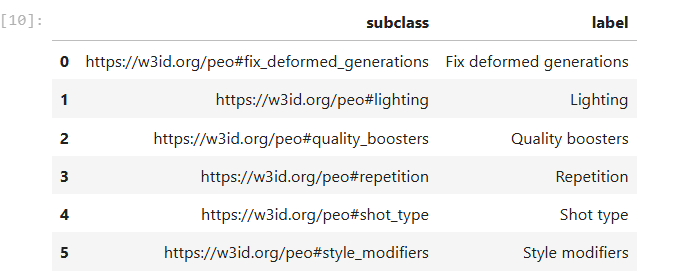
\includegraphics[width=0.9\linewidth]{Figures/fig_50.png}
    \caption{CQ4 SPARQL query results}
    \label{fig:enter-label}
\end{figure}
As expected, we get all the image prompting techniques in the ontology.\\

The fifth competency question \textbf{CQ5: What are code prompting techniques?} is translated into:
\begin{lstlisting}
SELECT DISTINCT ?subclass ?label
WHERE {
    ?subclass rdfs:subClassOf <https://w3id.org/peo#code_prompting> .
    OPTIONAL { ?subclass rdfs:label ?label . }
}  
\end{lstlisting}
Getting the following results:
\begin{figure}[H]
    \centering
    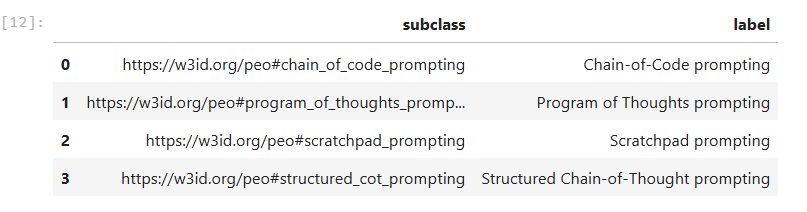
\includegraphics[width=0.9\linewidth]{Figures/fig_51.png}
    \caption{CQ5 SPARQL query results}
    \label{fig:enter-label}
\end{figure}
The table contains, as expected, all the code prompting techniques in the ontology.\\

The sixth competency question \textbf{CQ6: Which task does a prompt solve?} is translated into:
\begin{lstlisting}
SELECT DISTINCT ?prompt ?task ?taskLabel
WHERE {
    ?prompt <https://w3id.org/peo#solves> ?task .
    OPTIONAL { ?task rdfs:label ?taskLabel . }
}
\end{lstlisting}
Getting the following results:
\begin{figure}[H]
    \centering
    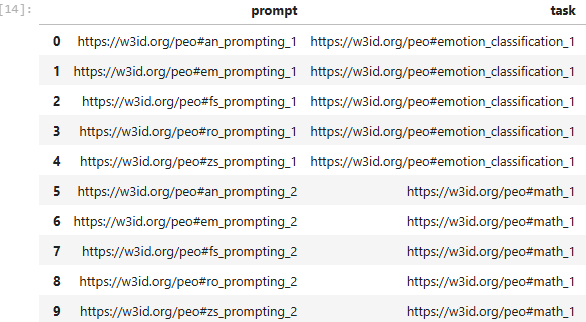
\includegraphics[width=0.9\linewidth]{Figures/fig_52.png}
    \caption{CQ6 SPARQL query results}
    \label{fig:enter-label}
\end{figure}
The table contains, as expected, all the prompts that solve tasks.\\

The seventh competency question \textbf{CQ7: Which prompts are generated using a prompting technique?} is translated into:
\begin{lstlisting}
SELECT DISTINCT ?prompt ?technique ?techniqueLabel
WHERE {
    ?prompt <https://w3id.org/peo#prompt_generated_using> ?technique .
    OPTIONAL { ?technique rdfs:label ?techniqueLabel . }
}
\end{lstlisting}
Getting the following results:
\begin{figure}[H]
    \centering
    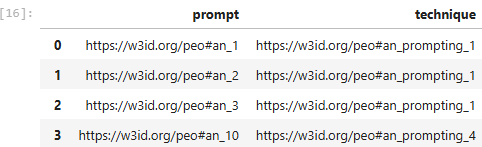
\includegraphics[width=0.9\linewidth]{Figures/fig_53.png}
    \caption{CQ7 SPARQL query results}
    \label{fig:enter-label}
\end{figure}
The complete table, as expected, contains all the prompt instances generated using instances of prompting techniques.\\

The eighth competency question \textbf{CQ8: What are the responses that follow each prompt?} is translated into:
\begin{lstlisting}
SELECT DISTINCT ?prompt ?response
WHERE {
    ?response <https://w3id.org/peo#response_followedby_prompt> ?prompt .
}    
\end{lstlisting}
Getting the following results:
\begin{figure}[H]
    \centering
    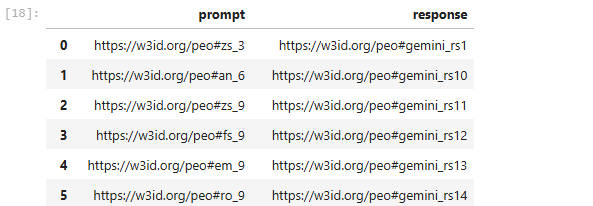
\includegraphics[width=0.9\linewidth]{Figures/fig_54.png}
    \caption{CQ8 SPARQL query results}
    \label{fig:enter-label}
\end{figure}
The complete table contains, as expected, all the responses of all prompt instances.\\

The ninth competency question \textbf{CQ9: What are possible tasks?} is translated into:
\begin{lstlisting}
SELECT DISTINCT ?task ?label
WHERE {
    ?task rdf:type owl:Class .
    ?task rdfs:subClassOf* <https://w3id.org/peo#task> .
    OPTIONAL { ?task rdfs:label ?label . }
}    
\end{lstlisting}
Getting the following results:
\begin{figure}[H]
    \centering
    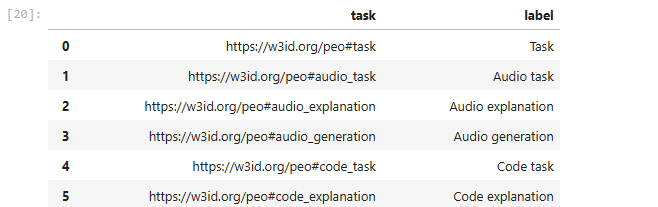
\includegraphics[width=0.9\linewidth]{Figures/fig_55.png}
    \caption{CQ9 SPARQL query results}
    \label{fig:enter-label}
\end{figure}
As expected, in the completed table we get all the possible task represented in the ontology.\\

The tenth competency question \textbf{CQ10: Which tasks are related to the text?} is translated into:
\begin{lstlisting}
SELECT DISTINCT ?task ?label
WHERE {
    ?task rdf:type owl:Class .
    ?task rdfs:subClassOf* <https://w3id.org/peo#text_task> .
    OPTIONAL { ?task rdfs:label ?label . }
}
\end{lstlisting}
Getting the following results:
\begin{figure}[H]
    \centering
    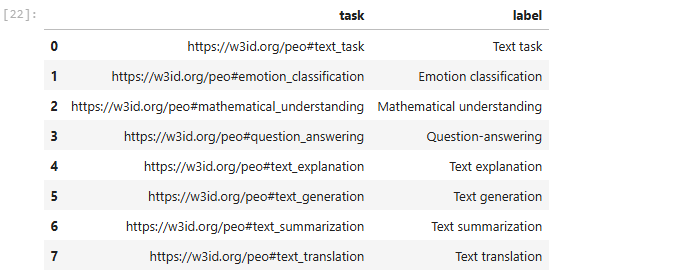
\includegraphics[width=0.9\linewidth]{Figures/fig_56.png}
    \caption{CQ10 SPARQL query results}
    \label{fig:enter-label}
\end{figure}

The resulting table, as expected, contains, all the task related to text.\\

The eleventh competency question \textbf{CQ11: What is a chat?} is translated into:
\begin{lstlisting}
SELECT DISTINCT ?property ?value
WHERE {
    <https://w3id.org/peo#chat> ?property ?value .
}
\end{lstlisting}
Getting the following results:
\begin{figure}[H]
    \centering
    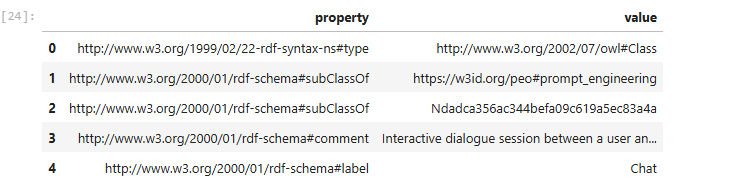
\includegraphics[width=0.9\linewidth]{Figures/fig_57.png}
    \caption{CQ11 SPARQL query results}
    \label{fig:enter-label}
\end{figure}
The result, as expected, is the definition of Chat.\\

The twelfth competency question \textbf{CQ12: What is a large language model?} is translated into:
\begin{lstlisting}
SELECT DISTINCT ?property ?value
WHERE {
    <https://w3id.org/peo#large_language_model> ?property ?value .
}
\end{lstlisting}
Getting the following results:
\begin{figure}[H]
    \centering
    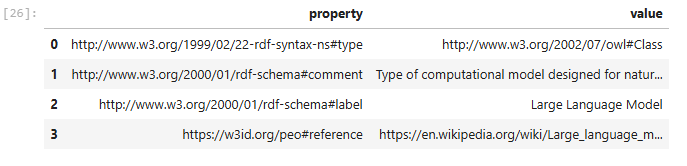
\includegraphics[width=0.9\linewidth]{Figures/fig_58.png}
    \caption{CQ12 SPARQL query results}
    \label{fig:enter-label}
\end{figure}
The result, as expected, is the definition of Large Language Model.\\

The thirteenth competency question \textbf{CQ13: What types of large language models are available?} is translated into:
\begin{lstlisting}
SELECT DISTINCT ?type ?label
WHERE {
    ?type rdfs:subClassOf <https://w3id.org/peo#large_language_model> .
    OPTIONAL { ?type rdfs:label ?label . }
}
\end{lstlisting}
Getting the following results:
\begin{figure}[H]
    \centering
    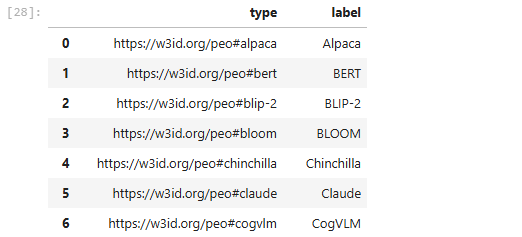
\includegraphics[width=0.9\linewidth]{Figures/fig_59.png}
    \caption{CQ13 SPARQL query results}
    \label{fig:enter-label}
\end{figure}
The resulting complete table, as expected, is the collection of all large language models represented in the ontology.\\

The fourteenth competency question \textbf{CQ14: What are large language models architectures?} is translated into:
\begin{lstlisting}
SELECT DISTINCT ?type ?label
WHERE {
    ?type rdfs:subClassOf <https://w3id.org/peo#base_model> .
    OPTIONAL { ?type rdfs:label ?label . }
}   
\end{lstlisting}
Getting the following results:
\begin{figure}[H]
    \centering
    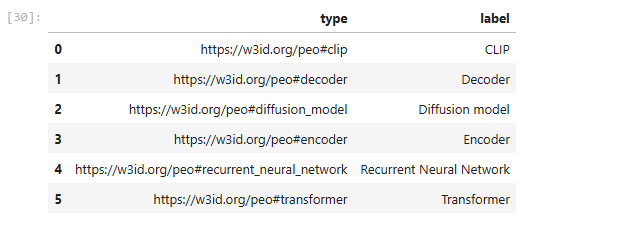
\includegraphics[width=0.9\linewidth]{Figures/fig_60.png}
    \caption{CQ14 SPARQL query results}
    \label{fig:enter-label}
\end{figure}
The result, as expected, is the collection of main large language models architectures.\\

The fifteenth competency question \textbf{CQ15: What are large language models capabilities?} is translated into:
\begin{lstlisting}
SELECT DISTINCT ?type ?label
WHERE {
    ?type rdfs:subClassOf <https://w3id.org/peo#capability> .
    OPTIONAL { ?type rdfs:label ?label . }
}
\end{lstlisting}
Getting the following results:
\begin{figure}[H]
    \centering
    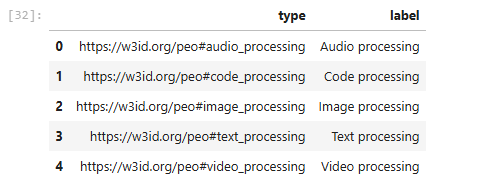
\includegraphics[width=0.8\linewidth]{Figures/fig_61.png}
    \caption{CQ15 SPARQL query results}
    \label{fig:enter-label}
\end{figure}
As expected, the results is the collection of all the capabilities represented in the ontology.\\

The sixteenth and last competency question \textbf{CQ16: What companies develop large language models?} is translated into:
\begin{lstlisting}
SELECT DISTINCT ?company ?label
WHERE {
    ?company rdf:type <https://w3id.org/peo#company> .
    OPTIONAL { ?company rdfs:label ?label . }
}
\end{lstlisting}
Getting the following results:
\begin{figure}[H]
    \centering
    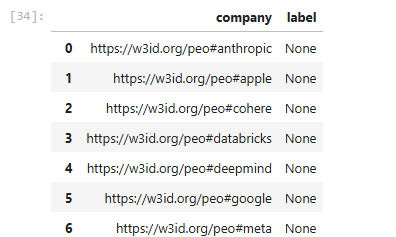
\includegraphics[width=0.8\linewidth]{Figures/fig_62.png}
    \caption{CQ16 SPARQL query results}
    \label{fig:enter-label}
\end{figure}
The result, as expected, is the collection of companies that develop large language models.\\
I proceed also, to execute SPARQL queries on the second version of PEO, the one that has been populated automatically using GPT-4. For obvious reasons, I am going to translate only competency questions that match changes introduced by the LLM. This because, as seen in the previous sections, GPT-4 does not introduce in the new version so much difference from the original version of PEO populated manually and if I execute all the competency questions, on the majority of them I would get the same results. Competency questions chosed for translation are four: CQ1, CQ2, CQ3 and CQ9.\\
The first competency question \textbf{CQ1: What is prompt engineering?} is translated into:
\begin{lstlisting}
SELECT DISTINCT ?property ?value
WHERE {
    <https://w3id.org/peo#PromptEngineering> ?property ?value .
} 
\end{lstlisting}
Getting the following result:
\begin{figure}[H]
    \centering
    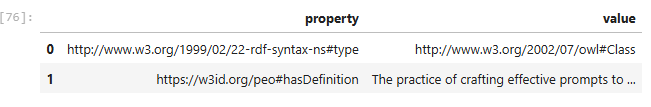
\includegraphics[width=0.9\linewidth]{Figures/fig_69.png}
    \caption{CQ1 SPARQL query results - PEO updated}
    \label{fig:enter-label}
\end{figure}

The second competency question \textbf{CQ2: What is a prompt?} is translated
into:
\begin{lstlisting}
SELECT DISTINCT ?property ?value
WHERE {
    <https://w3id.org/peo#Prompt> ?property ?value .
}
\end{lstlisting}
Getting the following result:
\begin{figure}[H]
    \centering
    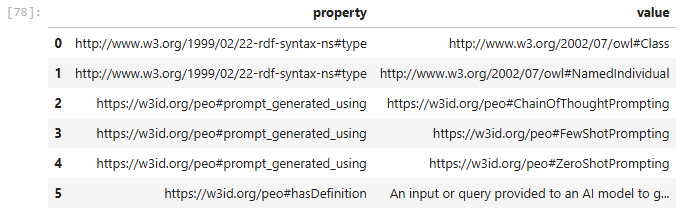
\includegraphics[width=0.9\linewidth]{Figures/fig_70.png}
    \caption{CQ2 SPARQL query results - PEO updated}
    \label{fig:enter-label}
\end{figure}

The third competency question \textbf{CQ3: What are prompting techniques?}
is translated into:
\begin{lstlisting}
SELECT DISTINCT ?instance
WHERE {
  ?instance <http://www.w3.org/1999/02/22-rdf-syntax-ns#type> <https://w3id.org/peo#PromptingTechnique> .
}
\end{lstlisting}
Getting the following result:
\begin{figure}[H]
    \centering
    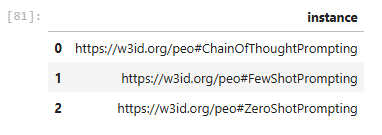
\includegraphics[width=0.7\linewidth]{Figures/fig_71.png}
    \caption{CQ3 SPARQL query results - PEO updated}
    \label{fig:enter-label}
\end{figure}

The ninth competency question \textbf{CQ9: What are possible tasks?} is translated
into:
\begin{lstlisting}
SELECT DISTINCT ?instance
WHERE {
  ?instance <http://www.w3.org/1999/02/22-rdf-syntax-ns#type> <https://w3id.org/peo#Task> .
}
\end{lstlisting}
Getting the following result:
\begin{figure}[H]
    \centering
    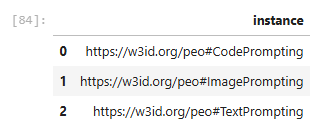
\includegraphics[width=0.6\linewidth]{Figures/fig_72.png}
    \caption{CQ9 SPARQL query results - PEO updated}
    \label{fig:enter-label}
\end{figure}

I specifically crafted the SPARQL queries to request the classes and instances added by ChatGPT in order to obtain different results; otherwise, I would have obtained the same results as before, since all the instances and classes added by the model are already present in the ontology.


\newpage
\section{Ontology publication and maintenance}
\label{section:4_5_publication}
The last step after the Ontology implementation in the LOT methodology is the Ontology publication phase, which scope is to provide an online ontology accessible both as human-readable documentation and a machine-readable documentation from its URI. This phase is divided into three sub-activities:
\begin{enumerate}
    \item \textbf{Propose release candidate}
    \item \textbf{Ontology documentation}
    \item \textbf{Online publication}
\end{enumerate}
as we can see in the figure below:
\begin{figure}[H]
    \centering
    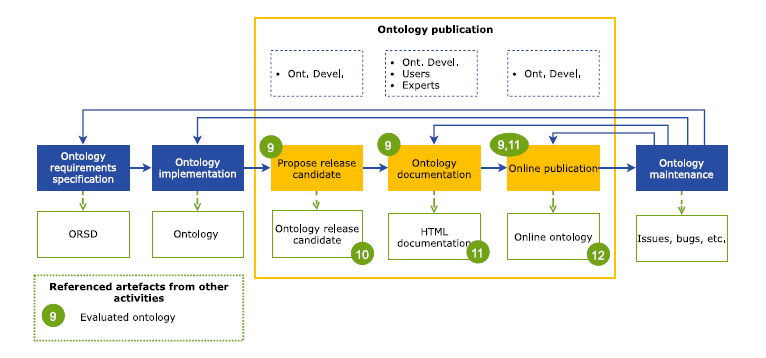
\includegraphics[width=0.9\linewidth]{Figures/fig_25.png}
    \caption{Ontology publication workflow}
    \label{fig:enter-label}
\end{figure}

\subsection{Propose release candidate}
\label{subsection:4_5_1_release}
After all the implementation and evaluation, in this step there is the decision about which version of the ontology is going to be published. It is a quite easy choice because, as said in pervious sections, the version populated automatically did not added any useful information from the original version. Moreover it added, according the OOPS! report, more pitfalls (five vs three) so the ontology that is going to be published is the 1.0 version of PEO, populated manually without any llm intervention.
\subsection{Ontology documentation}
\label{subsection:4_5_2_docs}
The ontology documentation is generated using Protegé and the OWLdoc plug-in which automatically generate HTML documentation starting from ontology code. The output of OWLdoc is the following:
\begin{figure}[H]
    \centering
    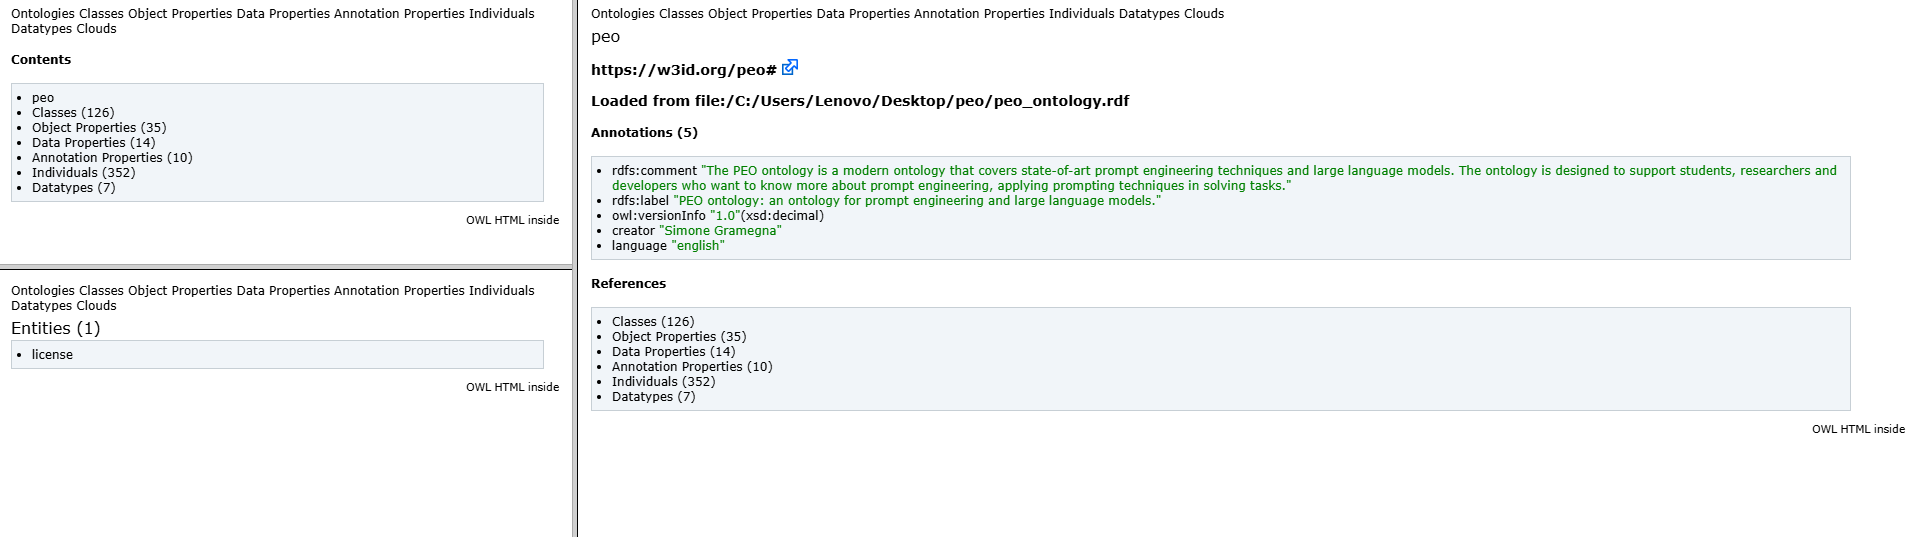
\includegraphics[width=0.9\linewidth]{Figures/fig_63.png}
    \caption{OWLdoc output}
    \label{fig:enter-label}
\end{figure}
The OWLdoc is available in the Github repository \href{https://github.com/simonegramegna/peo/tree/main/docs}{here} in the \textit{/docs} folder and it can be consulted online \href{https://peoontology.vercel.app/}{here}. The documentation is made accessible for everyone using Vercel: a cloud platform for hosting web applications and static sites. This free service using an integrated Github action, takes as input the documentation in the repository and publishes online automatically without requiring any effort by the developer. The \textit{official documentation website} is:
\href{https://peoontology.vercel.app/}{https://peoontology.vercel.app/}.

\subsection{Online publication}
\label{subsection:4_5_3_publication}
Once the ontology documentation is ready, the ontology can be published online on major vocabularies repository, by accessing the ontology using its URI. I will consider two most known repositories for ontology publishing: \href{https://w3id.org/}{w3id.org} and \href{https://bioportal.bioontology.org/}{BioPortal}.

W3id.org a permanent identifier service that provides stable, persistent, and HTTP-resolvable URIs for web resource. The creation of a new identifier for publishing a new ontology is made using Github and the official W3id.org Github repository. The procedure followed is straightforward, first I fork the W3id.org Github repository on my Github, creating a "copy" of the repository. 
\begin{figure}[H]
    \centering
    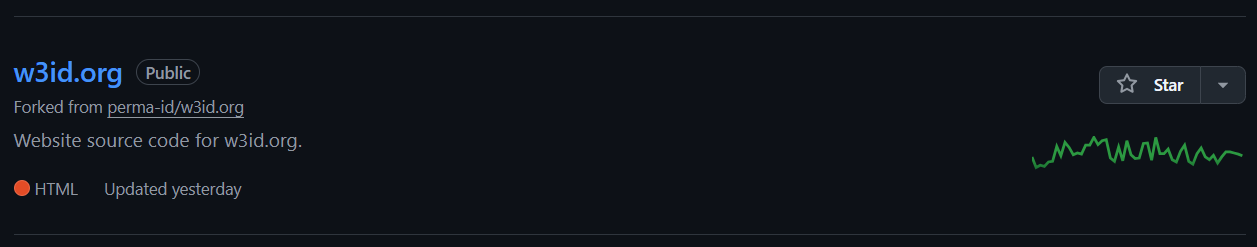
\includegraphics[width=0.9\linewidth]{Figures/fig_65.png}
    \caption{Forked W3id.org repository}
    \label{fig:enter-label}
\end{figure}
Then I create a new branch and I create a new directory with the intended permanent identifier name, in my case I create a directory called \textit{"peo"}. Inside this directory I create two files:
\begin{itemize}
    \item \textit{README.md:} contains more identifier info and contact info, for human to read.
    \item \textit{.htaccess:} contains redirection rules, for computer to read and perform.
\end{itemize}
In the case of PEO, the \textit{README.md} contains all my contact information with the link to the peo Github repository while the \textit{.htaccess} contains the following redirections rules:
\begin{lstlisting}
# Activates Rewrite Engine
RewriteEngine On

# Content negotiation for RDF/XML
RewriteCond %{HTTP_ACCEPT} application/rdf\+xml
RewriteRule ^$ https://raw.githubusercontent.com/simonegramegna/peo/refs/heads/main/peo_ontology.rdf [R=303,L]

# Content negotiation for Turtle
RewriteCond %{HTTP_ACCEPT} text/turtle
RewriteRule ^$ https://raw.githubusercontent.com/simonegramegna/peo/refs/heads/main/peo_ontology.ttl [R=303,L]

# Default: serves HTML for browser or client not RDF-aware
RewriteRule ^$ https://peoontology.vercel.app/ [R=303,L]

# Blocks directory indexing
Options -Indexes
\end{lstlisting}
Once the two files are completed, I submitted a pull request to the main branch that is approved by one of repository administrators. As soon the merge of the created branch, it is possible to access to the ontology using its URI, in the case of PEO the URI is: \href{https://w3id.org/peo}{https://w3id.org/peo} bringing the user with an HTTP request to the online ontology documentation.
\begin{figure}[H]
    \centering
    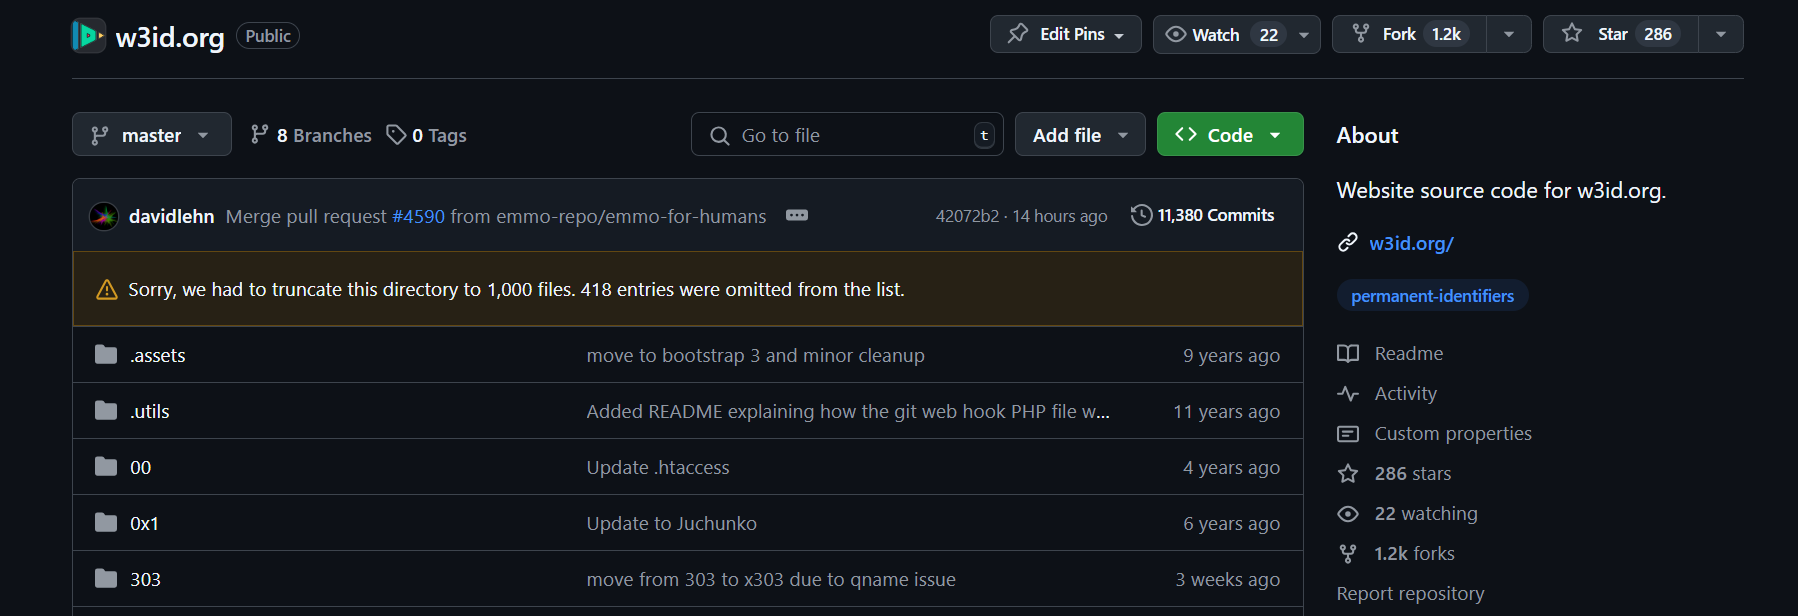
\includegraphics[width=0.9\linewidth]{Figures/fig_66.png}
    \caption{W3id.org repository main directory}
    \label{fig:enter-label}
\end{figure}

BioPortal is a  web-based platform designed for the management, exploration, and publication of biomedical ontologies, during the years it has become popular among ontology engineers choosing it as a repository for the publication of different types of ontologies not only in biomedical field. BioPortal offers developers a simple and intuitive interface to publish an ontology, providing the ability to track various versions and visits to the ontology. First I created an account on BioPortal and then I specified all the informations about the ontology: the version, the type (RDF) and the release date. I also specified my contact informations like the e-mail and the Github repository.
\begin{figure}[H]
    \centering
    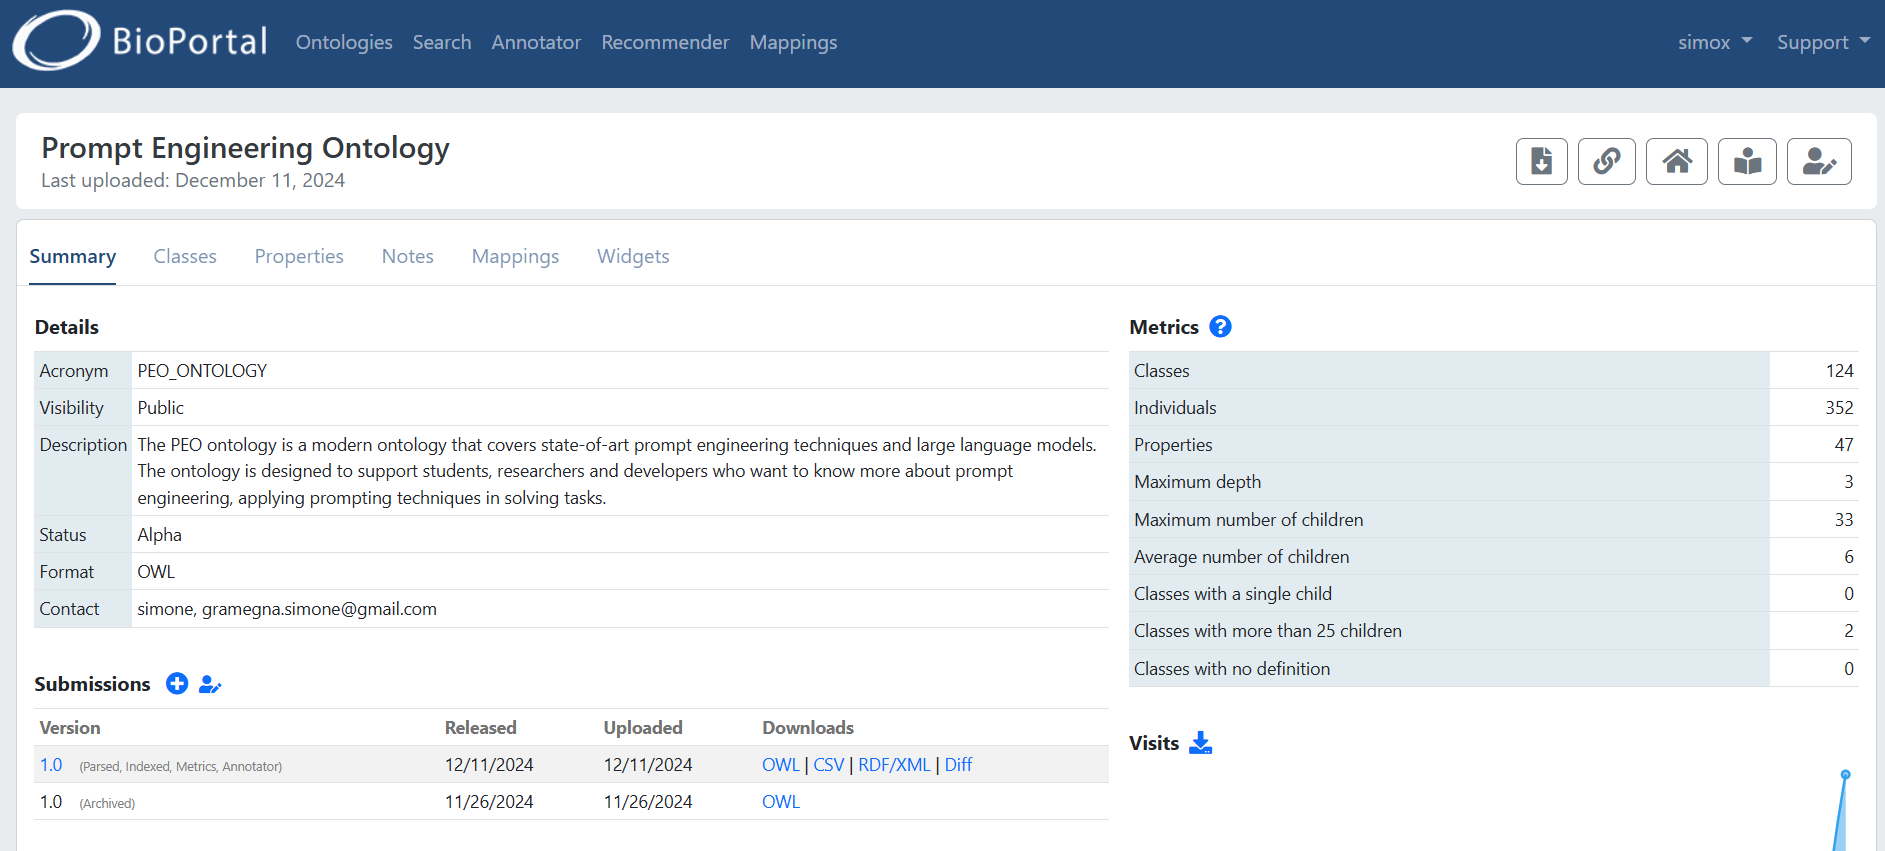
\includegraphics[width=0.9\linewidth]{Figures/fig_67.png}
    \caption{BioPortal main page}
    \label{fig:enter-label}
\end{figure}
The ontology is published at the link \href{https://bioportal.bioontology.org/ontologies/PEO_ONTOLOGY?p=summary}{here} and it is possible using the web interface view the whole ontology: classes, object properties, data properties and individuals. This is a very useful feature because the user has no need to download any additional software, moreover BioPortal computes automatically base ontology metrics. 
\begin{figure}[H]
    \centering
    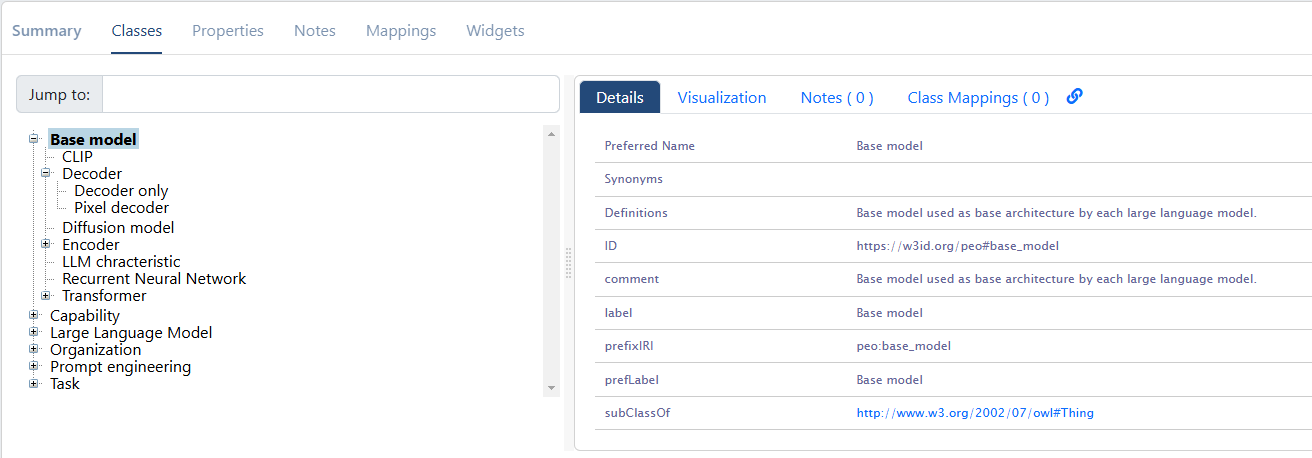
\includegraphics[width=0.9\linewidth]{Figures/fig_68.png}
    \caption{BioPortal ontology interface}
    \label{fig:enter-label}
\end{figure}


\newpage
\section{Ontology maintenance}
The ontology maintenance is the phase that concludes the iteration of the ontology development process, the goal of this phase is to update the ontology during its life cycle. This phase in the case of prompt engineering ontology is important, prompting techniques and large language models are constantly evolving, and regularly updating the ontology is essential to keep it aligned with the latest technologies introduced.\\
In cases where the necessary changes significantly alter the structure of the ontology, it is advisable to formulate new functional requirements through updated competency questions that align with the changes to be introduced. Changes may lead not only to updates but also to the introduction of bugs and pitfalls, which can be identified through the evaluation techniques previously discussed and resolving these issues ensures the quality of the ontology. In general, monitoring and maintaining the traceability of the requirements, bugs and suggestions identified in this activity allows storing discussions and decisions taken that can be later reused. The LOT methodology is designed to support those practices aligned with modern software engineering methodology like the agile methodology from whose iterativity it draws inspiration.

\begin{figure}[H]
    \centering
    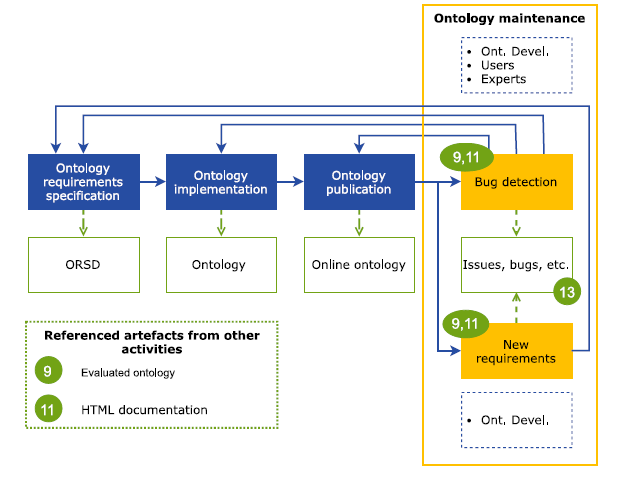
\includegraphics[width=0.9\linewidth]{Figures/fig_33.png}
    \caption{Ontology maintenance workflow}
    \label{fig:enter-label}
\end{figure}

\newpage
\section{Results discussion}
The design and implementation phases led the creation of an ontology that is the very first to comprehensively and exhaustively represent prompt engineering techniques and large language models. As discussed in previous chapters, resources on these topics are often quite limited and fragmented. So the PEO thus becomes an important reference in these fields providing users with a useful and effective tool to learn more about large language models and prompt engineering techniques.



\subsection{Evaluation results discussion}
The results obtained during the evaluation process of the PEO reveal important insights into its design, structure, and functionality. Through a combination of tools and methods, such as HermiT reasoner, OntoMetrics, and OOPS! validation, the ontology was rigorously assessed, highlighting both its strengths and areas for improvement.

\subsubsection{PEO strengths}
There are three main strengths of the PEO found during the evaluation:
\begin{enumerate}
    \item \textbf{Logical Consistency and Reasoning:} the HermiT reasoner confirmed that the ontology's logical structure is sound, with no inconsistencies detected in both the manually populated version and the updated version generated by GPT-4. The correct inference of disjoint classes and relationships indicates robust foundational design.

    \item \textbf{Expressiveness and Structural Metrics:} OntoMetrics demonstrated the ontology’s comprehensiveness, with 2684 axioms and SRIF(D) expressivity, supporting advanced reasoning while maintaining computational efficiency. The hierarchical organization (199 SubClassOf axioms) facilitates inheritance and scalability, and the inclusion of 352 individuals indicates practical applicability.

    \item \textbf{Semantic Coverage:} competency questions translated into SPARQL queries yielded expected results, confirming that the ontology effectively represents key concepts, such as prompting techniques, tasks, and the relationships between prompts and their generated responses. This shows that the ontology is well-aligned with its design goals.
\end{enumerate}
The PEO demonstrates strong logical consistency, comprehensive semantic coverage, and effective reasoning capabilities, supported by its well-structured hierarchy and expressiveness. These strengths validate its robustness as a tool for representing prompt engineering concepts and enabling practical applications.

\subsubsection{PEO limitations}
The evaluation found also the following limitations:
\begin{itemize}
    \item \textbf{Pitfalls in Structure and Usability:} OOPS! detected structural and usability issues, such as unconnected elements and missing annotations. These issues were more pronounced in the GPT-4-populated version, where newly introduced classes (e.g., Task, PromptingTechnique) lacked connections to the broader ontology. This indicates that automated population requires further refinement to align with ontology design principles.

    \item \textbf{Simplistic Relationships:} metrics such as low relationship richness (0.160338) suggest that the ontology is more focused on defining concepts than on establishing interconnections. While this simplifies reasoning, it may limit the representation of complex semantic relationships.

    \item \textbf{Underutilized Properties:} object and data property axioms reveal limited use of features such as functional, symmetric, or inverse properties. Incorporating these could enhance the ontology's ability to model constraints and unique relationships.

    \item \textbf{Inconsistencies in Naming Conventions:} the naming conventions of new classes in the other version of PEO introduced by GPT-4 deviated from the original ontology’s standards, potentially affecting usability and integration.
\end{itemize}
In general, the major issues are present in the version of the PEO populated using GPT-4, as, as previously observed, it has not proven capable of correctly populating the original version of the ontology with new instances. Regarding the original version of the PEO, there are solvable pitfalls, which I will discuss in the next section.

\subsection{PEO pitfall correction}

Considering the limitations outlined in the previous section, caused by the pitfalls in the main version of the PEO, I proceed to address and correct the identified pitfalls:
\begin{itemize}
    \item \textbf{P04 - Creating unconnected ontology elements:} this pitfall involves the \textit{prompt\_engineering} class which has no relation with any other class in the ontology.

    \item \textbf{P34 - Untyped class:} this pitfall involves elements in SWRL rules.

    \item \textbf{P41 - No license declared:} this pitfall is due to the absence of the license in the ontology.
\end{itemize}
The resolution of these pitfalls is essential to enhance the quality of the published ontology.

\subsubsection{P04 resolution}
This pitfall, as said before, involves the \textit{prompt\_engineering} class which has no relation with any other class in the ontology, this because the \textit{prompt\_engineering} is a sort of "container" of classes related to prompt. In order to connect \textit{prompt\_engineering} I created the object property \textit{applied\_to} (with inverse relation \textit{supports}) which connects \textit{prompt\_engineering} with the \textit{large\_language\_model} class.

\begin{figure}[H]
    \centering
    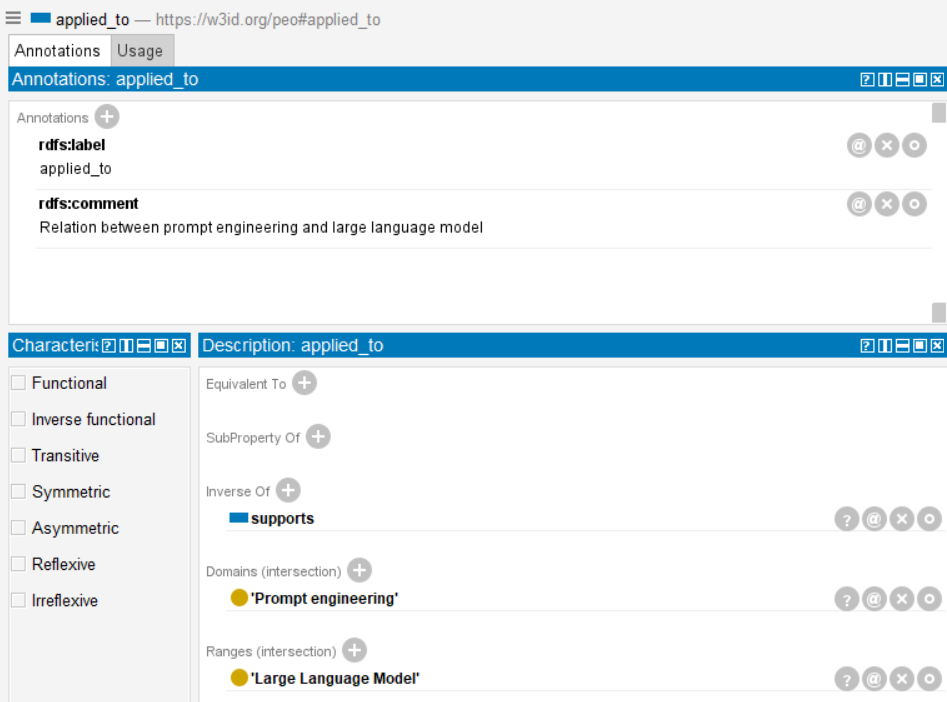
\includegraphics[width=0.7\linewidth]{Figures/fig_78.png}
    \caption{Object property between Prompt Engineering class and Large Language Model class}
    \label{fig:enter-label}
\end{figure}

\subsubsection{P34 resolution}
It is impossible to solve this pitfall because the affected elements are automatically created by Protegé when I define a SWRL rule. In fact SWRL is not part of the OWL languages so the types of the variables are not recognized. To address this issue, I have decided to remove the SWRL rules and replace them with property chains available in OWL. In this way, it is possible not only to reduce complexity, as SWRL rules involve a non-negligible computational cost, but also to make the ontology more portable, given that not all reasoners support SWRL rules.\\
In this case, I replaced the SWRL rule:
\begin{lstlisting}
peo:develops(?c, ?x) ^ peo:has_variant(?x, ?y) -> peo:develops(?c, ?y)
\end{lstlisting}
with the following object property chain:
\begin{figure}[H]
    \centering
    
\includegraphics[width=0.7\linewidth]{Figures/fig_81.png}
    \caption{Object property chaining for develops}
    \label{fig:enter-label}
\end{figure}
The same approach is applied to the other object properties. A particular case is the SWRL rule S2: 
\begin{lstlisting}
peo:evolves(?x, ?y) -> peo:has_variant(?x, ?y)
\end{lstlisting}
In which, instead of using the property chain, I define it directly as an object property \textit{evolves} as sub property of \textit{has\_variant} as we can see in the figure below:
\begin{figure}[H]
    \centering
    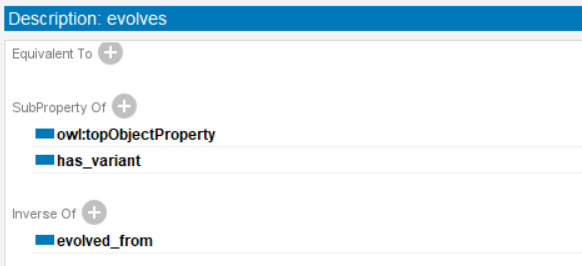
\includegraphics[width=0.9\linewidth]{Figures/fig_82.png}
    \caption{evolves object property}
    \label{fig:enter-label}
\end{figure}
When the HermiT reasoner is activated, the inferences derived from the property chains are equivalent to those produced by the SWRL rules.

\subsubsection{P41 resolution}
This pitfall, as said before, s due to the absence of the license in the ontology. In order to solve this pitfall, I created the annotation property \textit{dcterms:license} taking inspiration from the paper \textit{"Malaysian Food Composition Ontology Evaluation"}\cite{yusof2019malaysian} and adding as ontology annotation the link of the license (GNU General Public License v3) as we can see in the figure below:
\begin{figure}[H]
    \centering
    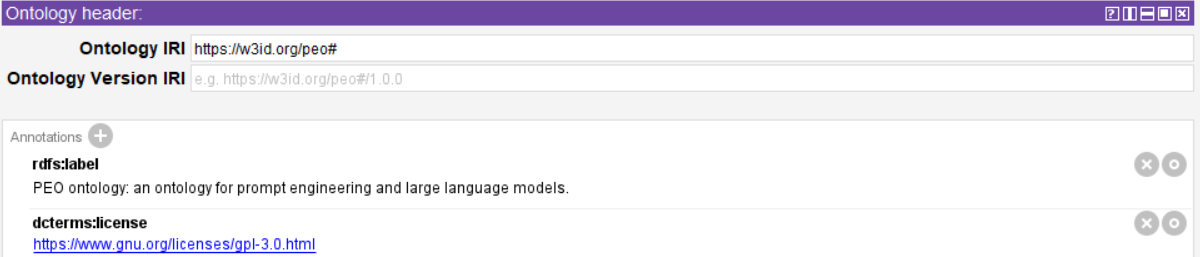
\includegraphics[width=0.9\linewidth]{Figures/fig_79.png}
    \caption{License annotation in PEO}
    \label{fig:enter-label}
\end{figure}
To solve this pitfall, instead of using software license like GNU General Public License, I used the Creative Commons license available at this link: \href{https://creativecommons.org/licenses/by/4.0/}{https://creativecommons.org/licenses/by/4.0/}.

\subsubsection{Minor changes in PEO}
During the revision phase, it has been noted that class, object properties and data properties name do not follow the Semantic Web naming conventions that establishes Camel Case for class names, with the first letter in upper case while for object properties and data properties the Camel Case is used but the first letter is in lower case. For example the object property \textit{evolved\_from} with this modification, it becomes \textit{evolvedFrom} and the \textit{large\_language\_model} class becomes \textit{LargeLanguageModel}. This modification took time, because the operation is made manually, but it ensures the quality and the compliance of the ontology to the semantic web standards.


\subsubsection{Final thoughts}
In the Introduction chapter there were two main questions:
\begin{enumerate}
    \item \textbf{Question 1: Is it possible to formalize the knowledge related to large language models and prompting techniques?}

    \item \textbf{ Is it possible to use the model formalization to get additional knowledge?}
\end{enumerate}

At the end of the experimentation, it is possible to give an answer to those two questions. The answer to the \textbf{question 1}, is: \textbf{yes}. During the whole process of the thesis starting from the state of art to the design and implementation I collected informations from different information sources like: papers, websites, Github repositories and then I gave a structure to all of this information, selecting important informations and entities useful for my scope and ignoring informations that are too specific or anyway useless for my scope. The process of design starting from selected informations added more specific information useful to give the direction of the implementation process of the ontology. During the implementation using Protege and owl it was possible to express all the concept that were defined theoretically or using schemes and the evaluation process gave me the assurance that all the development process produced the desiderated result. So yes, it is possible to formalize the knowledge related to large language models and prompting techniques and it has been successfully made.\\
Also the answer to the \textbf{question 2} is yes, because using the inference mechanism and property chaining defined in the PEO it is possible to get informations about all the characteristics of each large language model represented and the connections with prompts generated using prompt engineering techniques. Complex rules are encoded into owl property chains so it is possible to get inferences using any reasoner available. 



Despite these minor issues, the PEO is well-designed, comprehensive, well-documented, and has very few problems. It significantly outperforms state-of-the-art ontologies related to large language models and prompt engineering.